\setcounter{chapter}{-1}
%%%%%%%%%%%%%%%%%%%%%%%%%%
\chapter{Proposal Summary}
%%%%%%%%%%%%%%%%%%%%%%%%%%

This chapter will not be part of the final thesis but serves as more of an executive summary of where I am in the thesis process.
\Cref{tab:timeline} describe the notional timeline of my doctoral work.
The following to sections briefly summarize the papers I have completed so far, and the papers that I plan to publish to complete my thesis.
More substantial descriptions of the work are given in the body of thesis.


\begin{table}
  \centering
  \begin{tabular}{lll}
  \toprule
  2019  & August            & Began research master's degree (CMU) \\
  2021  & August            & Completed masters, began PhD \\
  % 2024  & July--September   & XferBench eval (\Cref{ch:hpo}) \\
  2025  & January           & Proposal \\
        & January--March    & Rich corpora (\Cref{ch:rich-corpora}) \\
        & April--June       & Morphemes (\Cref{ch:morphemes}) \\
        & July--September   & Morpheme structure (\Cref{ch:syntax}) \\
        & September         & Defense \\
  \bottomrule
  \end{tabular}

  \caption{Timeline of proposed work and thesis completion.}
  \unskip\label{tab:timeline}
\end{table}

\section{Completed Work}
% The following completed research papers will be incorporated into the thesis (either in part or their entirety).
% Other work has be published and/or completed during the course of my master's and doctoral work but will not play major role in the thesis.


\subsection{Recommendations for Systematic Research on Emergent Language}
\noindent
\citet{boldt2022recommendations} was rejected from ICML 2022; part of this work was expanded into ``A Review of the Applications of Deep Learning-Based Emergent Communication'' discussed below.
This is a position paper which critiques and makes recommendations for emergent communication research from a meta-scientific angle.
It begins by specifying the goals of emergent communication research (which would eventually become the TMLR paper).
In light of these goals, which are split between ``engineering'' and ``scientific'' goals, the paper discusses core methodological elements of engineering and science.
Finally, each of the core methodological elements is explicitly detailed in the context of emergent communication.
In addition to the goals, the particular elements of engineering which are pursued in this thesis are evaluation metrics and standard datasets.

\subsection{A Review of the Applications of Deep Learning-Based Emergent Communication}

\noindent
\citet{boldt2024review} was published in the \textit{Transactions of Machine Learning Research} (TMLR) in February 2024.
This paper comprehensively reviews the applications and goal of emergent communication research drawing on both the literature and the author's (i.e., Brendon and David's) experience in the field.
Each application, in addition to a description and review of the relevant literature, is a accompanied by a brief set of recommendations on the most fruitful next steps for that research direction.
The set of applications themselves is divided into three categories:
  (1) internal applications, which focus on improving the methods of emergent communication itself,
  (2) task-driven applications, which look at engineering tasks focused on more effectively solving particular problems,
  and (3) knowledge-driven applications, which aim at increasing scientific understanding of particular phenomena.

\subsection{XferBench: a Data-Driven Benchmark for Emergent Language}
\noindent
\citet{boldt2024xferbench} was published in the \textit{Proceedings of the 2024 Conference of the North American Chapter of the Association for Computational Linguistics: Human Language Technologies (Volume 1: Long Papers)} (NAACL).
This paper introduces a first-of-its-kind evaluation metric/benchmark for emergent languages.
It addresses the question of the \emph{quality} of an emergent language by looking at its similarity to human language from a data-driven, machine learning perspective.
Specifically, it quantifies ``similarity to human language''---and, therefore, overall quality---as how much pretraining on an emergent language corpus improves performance on modeling human language (although we also test machine translation).
XferBench is published as an easy-to-use Python package, and since it only requires an unannotated corpus of utterances from the emergent language, it is intended to have widespread use in emergent communication research.


\subsection{ELCC: the Emergent Language Corpus Collection}
Under review at the \textit{2024 Conference on Neural Information Processing Systems Datasets and Benchmarks Track} (decision in September 2024).
This paper introduces a collection of over $70$ emergent language corpora from across $8$ different systems in the literature.
Each of these corpora is annotated with statistical analyses as well as metadata documenting the features of the system/environment it came from.
Such a resource is intended to make studying emergent languages themselves far easier since it obviates the need run the systems oneself and enable comparative studies given the variety of emergent communication systems included.

\subsection{Other Work}
Some work completed during the course of master's and doctoral work will not factor heavily into the thesis.
In ``Mathematically modelling the lexicon entropy of emergent language'' \citep{boldt2022mathematically}, we investigate using a formal model based on the Chinese restaurant process to make predictions of the entropy of lexica in emergent languages; this is intended to be a sort of exemplar of using formal models to make clear, determinate hypotheses regarding emergent communication experiments.
In ``Shaped rewards bias emergent language'' \citep{boldt2022shaped}, we argue that reward shaping (a common feature of reinforcement learning experiments) has the potential to bias (i.e., predetermine) properties of the resulting emergent language.
In ``Case study: deontological ethics in NLP'' \citep{prabhumoye-etal-2021-case}, we apply deontological approach to ethics to different real-world scenarios in natural language processing-based systems.



\section{Proposed Work}
This section will briefly described the proposed work for the completion of the doctoral thesis.
Each of these papers is intended to a standard conference-length paper (i.e., 8--9 pages).

\subsection{XferBench analysis}
In this paper, which is currently in progress, we will run XferBench on all of the languages in ELCC in order to find correlations between XferBench performance and features of the corpora and emergent communication system they come from.
For example, we hope to answer question such as ``Do more complex environments yield better emergent languages?'' or ``Is token entropy of an emergent language predictive of its score on XferBench?''
These analyses will help to understand what XferBench is measuring and whether it is easily explainable by surface-level statistics of the corpus or whether some deeper structural characteristics might be required to understand XferBench's outputs.


\subsection{Rich emergent language corpora}
ELCC, the current collection of emergent language corpora, only includes the corpora themselves and aggregate statistics, but many interesting research directions require not only having access to the tokens of utterances themselves but also their context.
For example, anything related to semantics is going to require some way to determine what an utterance means.
Thus, we propose an extension to ELCC which takes the same set of corpora and includes information about the state of the environment before and after each utterance so as to supply grounding for each of the utterances.
From here, it will be possible to explore a far greater range of phenomena with respect to the emergent language corpora in ELCC\@.

\subsection{Automatically detecting morphemes in emergent language corpora}
While the original plan was to create a linguistic counterpart to XferBench, that is, some benchmark-like metric which measured the presence of human language-like linguistic structures in emergent communication, I rolled back my ambition considerably as there are not yet methods for detecting structure in emergent communication generally.
Thus, this project will make an important step in the direction of such a metric by introducing and testing an algorithm to detect and segment emergent communication utterances into morphemes: particular meanings paired with an atomic form.
Detecting morphemes is critical in building up to ``higher-level'' linguistic concepts like syntax and discourse, yet there are no existing methods determining what the meaningful units of an emergent communication utterance are in a general, system-agnostic way (e.g., is each token its own morpheme are they sub-morpheme units?).
This work will leverage the rich emergent language corpora discussed above as it is necessary to pair the utterances (form) with the accompanying context (meaning) in order to uncover morphemes (or at least an analogous structure).
Being able to turn emergent languages represented as strings of raw tokens into strings of morphemes will enable more principled research on linguistic structures which presuppose the existence and identification of morphemes (e.g., syntax).

\cmt{Add comment motivating morpheme detection by talking about double articulation and how parsing over characters would be absurd; you need a lex step first.}


\subsection{Automatically detecting morpheme structure}
Building on the above chapter detecting morphemes, this chapter will use a somewhat similar approach to detect structural features in emergent language corpora.
Namely, the strings of morphemes from the previous method are first mapped to classes (determined, mostly, by the semantics of the morphemes) which are then run through decision functions which detect structural features (i.e., one morpheme class succeeding another).
These structural features are then generalized into patterns (I would hesitate to call them ``rules'') using a statistical measure.
The algorithm, then, yields a list of the most frequent morpheme patterns found in the emergent language corpus.
This chapter stops short of claiming that what is being detected is ``syntax'' in any linguistically robust sense and instead focuses on a more minimalist notion of structure which can later be incorporated into more broad-reaching account of syntax (outside the scope of this thesis, though).

\cmt{Allude to recursive application of the algorithm in the chapter, although finding constituents or heads might be beyond the pay grade (still good for future work and contextualization, though).}



%%%%%%%%%%%%%%%%%%%%%%
\chapter{Introduction}
%%%%%%%%%%%%%%%%%%%%%%

Modern-day large language model-based AI systems are good a mimicking human language.
Some might even say they are good at \emph{using} human language, but this is either imprecise or inaccurate:
  LLMs' production of text is based the statistical likelihood of meaningless (so far as they are concerned) tokens, fine-tuned to humans' preferences.
This is in contrast to humans' use---and event more so their acquisition---of language which is laden with meaning derived from the rich internal, physical, and social context which permeates language use.
The end result is that LLMs' approximation of human language fails at a number of tasks, but, more significantly, falls short in providing insights into the nature of human language itself.
\cmt{Mention the data problem for LLMs.}

\emph{Emergent communication} (also known as \emph{emergent language}) is an alternative paradigm to developing language-capable models that does not does not train on human language data but rather invents a communication system \emph{de novo}.
In its most basic form, emergent communication comprises a simulation using neural network-based agents which are trained to cooperatively complete some task in a virtual environment.
These agents are equipped with a communication channel of discrete tokens with no \emph{a priori} meaning---the meaning of communication is established through the optimization process encouraging communication which is advantageous to completing the task.
% The communication protocol, then, is the ``emergent language'' since the meaningful system of communication as arisen organically from the environment and task.

Emergent communication differs from the more ``traditional'' approach to language that LLMs use in that it does not try mimic human language but instead tries to rederive language from similar function pressures which are hypothesized to have guided human language's own evolution.
Since the process language emerging is far more analogous to how human language develops and is learned, it has a much greater potential to yield significant gains the scientific understanding of human language.
Furthermore, certain practical tasks might lie beyond the reach of the mimicry approach LLMs employ due to surface-level operations; these problems, too, can be addressed by emergent communication which models not only the surface features of language but also its semantics and social context.

Here is the problem: the field of emergent communication has not yet solved any problems either in the area of scientific understanding nor in practical applications.
Furthermore, it has not even shown measurable progress towards these goals either.
This thesis, then, endeavors to establish principles and practices in emergent communication that permit and encourage measurable progress in the development of emergent languages specifically with the aim of helping emergent communication research achieve its potential in solving practical applications and improving scientific understanding.
\cmt{After this general description of the thesis give another, be more specific with a sentence.}

\section{Background}

The field of deep learning-based emergent communication has its genesis in 2016 with papers including
  ``Learning to communicate with deep multi-agent reinforcement learning'' \citep{foerster2016learning}
  and ``Multi-Agent Cooperation and the Emergence of (Natural) Language'' \citep{lazaridou2016multiagent}.
These were the first paper to combine combine deep learning, and specifically deep reinforcement learning, to developing discrete token-based communication systems from scratch.
While prior work applied mathematical models \citep{brighton2005} and classical machine learning methods \citep{werner_Dyer_1991}, the introduction of deep learning opened up the possibility of a far more robust notion of the results of the simulations being \emph{emergent}.
That is, with mathematical models the range of results is tightly constrained by the design of the model and ``emergent'' phenomena are either relatively simple or encoded into the model itself.\footnote{Although Conway's Game of Life is notable exception to this.}
Deep reinforcement learning, on the other hand, has demonstrated vivid example of complex behaviors emerging in environments with simple rules such as DeepMind's AlphaZero \citep{silver2017masteringchessshogiselfplay} or OpenAI's multi-agent hide-and-seek \citep{baker2020emergenttoolusemultiagent}.

The prototypical emergent communication experiment consists two or more deep neural network-based agents situated in some kind of environment or game where they must cooperate in order to succeed.
The agents are equipped with a communication channel consisting of discrete tokens with no \emph{a priori} meaning; it is only through the reinforcement learning-based optimization that messages passed between agents begin to take on meaning.
The resulting behavior, most especially the communication protocol, is the typically the object analysis, addressing question such as:
  Did an effective communication protocol emerge at all?
  What structural features characterize it?
  Do these features align at all to human language?
  What can we infer about language formation more generally from the above?
\cmt{Mention somewhere that the message is generated by a deep neural network.}

In practice, much of the literature has focused on the signalling game and the emergence of compositionality in communication (jointly and separately).
The signalling game was introduced in the context of game theory by David Lewis \citep{lewis1970ConventionAP}.
The signalling game is one of the simplest possible environments for emergent communication contributing, in large part, to its popularity.
It consists of only two agents: a sender and a receiver.
The sender makes on observation (e.g., an orange circle) and sends a message to the receiver who must, based on the message alone, determine the nature of the observation (e.g., it was an orange circle, not a blue circle).
A visualization of the signalling game is provided in \Cref{fig:signaling-game}.
\cmt{See such and such research for examples of these themes.}
The question of compositionality arises when we look at how the communication protocol encodes compound meanings like a red square: A compositional protocol would encode ``red'' and ``circle'' with their own words which could be reused to express meanings like a red circle or a blue square.
On the other hand, holistic communication sometimes emerges where a unique word refers to red square, bearing no relation to the word(s) for red circle.
Compositional communication, generally, is seen as more desirable both for practical reasons (more efficient encoding of information) as well as for its resemblance to how humans tend to encode meaning in language.

\begin{figure}
  \centering
  \begin{subfigure}[b]{0.53\textwidth}
    \centering
    \setlength\fboxsep{0pt}
    \def\cubeoffset{0.25}
\tikzset{
  boxface/.pic={
    \fill
      (0,0)
        edge (1,0)
        edge (0,1)
        edge (0-\cubeoffset,0+\cubeoffset)
      (1,1)
        edge (1,0)
        edge (0,1)
        edge (1-\cubeoffset,1+\cubeoffset)
      (0-\cubeoffset,1+\cubeoffset)
        edge (0-\cubeoffset,0+\cubeoffset)
        edge (1-\cubeoffset,1+\cubeoffset)
        edge (0,1)
      ;

    \fill (0.3, 0.7) circle [radius=0.03];
    \fill (0.7, 0.7) circle [radius=0.03];

    \path [] (0.3, 0.3) edge (0.7, 0.3);
  }
}

\begin{tikzpicture}[scale=0.8, transform shape]

  \node (t1) at (-4, 0.5) {\large$T_1$};
  \draw (-\cubeoffset,0) pic [xscale=-1] {boxface};
  \fill [orange!60] (-3, 0.5) circle [radius=0.4];
  \node at (-1.9, 0.5) {\Large\eye};
  \draw (3,0) pic {boxface};
  \draw [gray] (-3.5, -0.4) to (4.8, -0.4);

  { [yshift=-2cm]
    \node (t2) at (-4, 0.5) {\large$T_2$};
    \draw (-1,0) pic {boxface};
    \node[rectangle callout, draw, callout absolute pointer={(0.1,0.5)}] at (1.3,1) {3 14 1 59 2};
    \draw (4-\cubeoffset,0) pic [xscale=-1] {boxface};
    \draw [gray] (-3.5, -0.4) to (4.8, -0.4);
  }

  { [yshift=-4cm]
    \node (t3) at (-4, 0.5) {\large$T_3$};
    \draw (-1,0) pic {boxface};
    \draw (3,0) pic {boxface};
    \node (opt1) [fill=orange!60,regular polygon, regular polygon sides=4, inner sep=0.25cm] at (5.5, 1.5) {};
    \node (opt2) [fill=blue!60,below=0.5cm of opt1,circle,inner sep=0.25cm,anchor=center] {};
    \node (opt3) [fill=orange!60,below=0.5cm of opt2,circle,inner sep=0.25cm,anchor=center] {};
    \node [left=0.0cm of opt3,anchor=east,yshift=-1.5mm] {\Large\leftpointright};
  }

  \draw [-stealth, black!50, dashed] (t1) to (t2);
  \draw [-stealth, black!50, dashed] (t2) to (t3);

\end{tikzpicture}

    \vspace{1cm}
    \caption{%
      $T_1$: The sender (left) observes an object.
      $T_2$: The sender passes a message to the receiver (right).
      $T_3$: The receiver chooses from a handful of candidate objects.
    }
    \unskip\label{fig:boxface}
  \end{subfigure}
  \hfill
  \begin{subfigure}[b]{0.45\textwidth}
    \centering
    \tikzstyle{blockStyle}=[
  draw=black!50,
  text width=2.7cm,
  minimum width=2cm,
  text centered,
  rounded corners,
  font=\scriptsize,
]

\newcommand\blocktext[2]{\textsc{#1}\\{\color{black!70}#2}}

\begin{tikzpicture}
  [node distance=3mm, outer sep=0mm, inner xsep=-1mm]

  \node (obs) [blockStyle] {\blocktext{Observation}{vector}};
  \node (sender) [blockStyle,below=of obs.south] {\blocktext{Sender}{RNN conditioned on observation}};
  \node (message) [blockStyle,below=of sender.south] {\blocktext{Message}{sequence of one-hot vectors}};
  \node (distobs) [blockStyle,right=of message.east] {\blocktext{Candidate\\Observations}{set of vectors}};
  \node (n0) at ({$(message)!.5!(distobs)$} |- {message.south}) {};
  \node (receiver) [blockStyle,below=of n0] {\blocktext{Receiver}{RNN conditioned on message and observations}};
  \node (pred) [blockStyle,below=of receiver.south] {\blocktext{Prediction}{prob.\@ dist.\@ over observations}};
  \node (reward) [blockStyle,below=of pred.south] {\blocktext{Reward}{real value}};

  \draw [-stealth] (obs) to (sender);
  \draw [-stealth] (sender) to (message);
  \draw [-stealth] (message) to (receiver);
  \draw [-stealth] (distobs) to (receiver);
  \draw [-stealth] (receiver) to (pred);
  \draw [-stealth] (pred) to (reward);
  \draw [-stealth, bend left, dashed] (obs.east) to (distobs);
  \draw [-stealth, dashed, inner sep=0mm] (reward.west) to[looseness=0.8, out=135, in=225] (sender.south west);
  \draw [-stealth, dashed] (reward.west) to[looseness=1, out=135, in=225] (receiver.west);

  \clip (obs.west |- obs.north) rectangle (distobs.east |- reward.south);
\end{tikzpicture}

    \caption{Illustration of the technical architecture of the signaling game.}
    \unskip\label{fig:signaling-chart}
  \end{subfigure}
  \caption{%
    An illustration of the discrimination variant of the signaling game, one of the simplest and most common environments in emergent communication research.
  }
  \unskip\label{fig:signaling-game}
\end{figure}


Other environments do appear in the literature such as navigation tasks or dialogue-based games.
\cmt{citations}
In addition to compositionality, other phenomena have been the subject of investigation such as pragmatics, transfer learning, and the information theoretic properties of emergent language.
\cmt{citations}
While there are too many papers to summarize comprehensively here, I estimate that there are on the order of $200$ papers directly related to emergent communication.\footnote{Figure based on finding ${\sim}150$ papers during a comprehensive literature review in 2023.}
For a general review of the emergent communication literature, I recommend \citet{lazaridou2020emergentmultiagentcommunicationdeep}.

\section{Motivation}

In the seven or so years of deep learning-based emergent communication's existence, there has been little concrete progress in the field.
Much of the research has focused on addressing small-scale, isolated phenomena without a way to unify the findings into a broader understanding.
While normal science (as Kuhn terms it \citep{kuhn}) often proceeds by small, additive research contributions, emergent communication has not developed paradigm where the small contributions can truly add together.
One can read much of the literature on emergent communication, learn of many different trends that appeared in particular environments, and still largely have no idea why emergent languages look the way they do nor what they might look like in a new environment.
Furthermore, despite the potential for groundbreaking application sin natural language processing and linguistics, emergent communication has not yielded any substantial contributions either \cmt{cite TMLR paper}.
\cmt{Mention that EC is hard in general?}

This thesis is intended to make foundational contributions addressing the structural issues in emergent communication research that has resulted in this.
In particular, the overall intent of the thesis is to create quantitative evaluative methods which work across a wide variety of emergent communication environments in order to support a research and development workflow more like that of the rest of deep learning-based research.
Methods should yield \emph{quantitative} metrics to permit direct comparison of different systems, statistical analysis, and more automated methods of exploring emergent communication environments.
These methods must also be \emph{evaluative} since we a number that we can optimize for---a goal---not simply a number describing one aspect of a system that requires further interpretation.
Finally, this thesis looks to rest of deep learning research, especially in regards to structures like benchmarks and evaluation metrics, for inspiration because these factors are critical for its own success.
While the long-term development of emergent communication methods needs far more than just borrowing methods from deep learning, developing general-purpose evaluative tools is critical in unifying the research efforts of the field such that they can begin to progress in a tangible way.

\paragraph{An aside}
While the fundamental lack of progress has, from an early point, been the main focus of my doctoral research, I had to make a decision between two ways of addressing this problem: the ``scientific'' way and the ``engineering'' way.
The scientific approach would entail developing a theory of emergent communication which would enable progress by first creating a concrete, unified theory that research could contribute two, and second, by illuminating the most promising directions based on the predictions of the field.
Such an approach was addressed by my paper ``Mathematically Modeling the Lexicon Entropy of Emergent Language'' \citep{boldt2022mathematically} which was a sort of proof-of-concept for this approach, attempting to establish an empirically verifiable formal model of certain behaviors in emergent communication experiments.
Of the two approaches, this one certainly had (and has) more appeal to me, but I ultimately decided against it largely because I judged that it was not feasible.
In essence, the current paradigm of emergent communication research follows this approach (even if the scientific method is hardly employed explicitly), that is, trying to find general principles which can be empirically verified.
I think this paradigm fails in large part because emergent language is\dots\emph{emergent}!
No amount of adding up little parts is going to tell you ahead of time what is going to happen in the large-scale, so the idea would go.
If this is true, and my intuition pushes me in this direction, then emergent communication, \emph{qua} emergent phenomenon, is a matter of ``go big or go home'': scale up or pack up.\footnote{This sounds like a bitter lesson \citep{bitter-lesson}.}

This leads us to the engineering approach which might be summed up as: how to scale up intelligently.
This is the approach this thesis follows.
In contrast to the scientific approach, the engineering approach focuses on creating structures which allow research to try a wide variety of approaches and efficiently sift through the results to find the next handhold in the ascent.
Naturally, some degree of theoretical understanding is necessary to explore intelligently, but the threshold of understanding for guiding exploration is lower than what might typically be associated with scientific understanding or prediction.
Finally, from a practical standpoint, the engineering approach proved more tractable for writing a thesis: the intermediate papers more easily speak for themselves and making an immediate impact is far more feasible.


\section{Overview}

This thesis has three main parts:
The first comprises \Cref{ch:elcc,ch:rich-corpora}, which introduce a large collection of emergent language corpora and corresponding semantic annotations.
Second, \Cref{ch:xferbench,ch:hpo} introduce and showcase XferBench, a deep transfer learning-based evaluation metric for emergent language corpora.
Lastly, \Cref{ch:morphemes,ch:syntax} introduce methods for detecting linguistic structures in emergent language corpora.
Each of these parts largely stands on its own for the purposes of readability as well as their contributions.
Nevertheless, the entire thesis is intended to provide a coherent, multi-pronged approach to the problem of a lack of measurability of progress.


\subsection{Emergent Language Data Resources}
\Cref{ch:elcc,ch:rich-corpora} introduce an important data resource to emergent communication research: the Emergent Language Corpus Collection (ELCC), a collection of emergent language corpora with semantic annotations of utterances derived from a variety of free and open source emergent communication implementations.
Each of these corpora is accompanied by metadata describing statistical properties of the corpus, taxonomic properties of the environment it came from, and a turnkey shell script for reproducing the corpus (or developing a new one).
This collection of corpora is made a public such that it can be both easily used and contributed to by the broader research community.

In its own right, this collection is a significant contribution to emergent communication as it increases the accessibility of emergent language data both for researchers who might be able to generate the emergent languages themselves and those looking to compare a wide variety of emergent languages.
More importantly for the thesis, though, having a robust collection of emergent language corpora is necessary test, contextualize, and motivate the results of the following chapters.
The transfer learning-based metric discussed below takes emergent language corpora as input, and to demonstrate its utility in comparing various approaches to emergent communication, it needs to be applied to a wide variety of emergent languages.
For the methods of detecting linguistic structure, not only is the variety of emergent languages important, but the semantic annotations are a critical part of discovering the latent structure that might be present in the emergent languages.
Thus, the collection of emergent language corpora forms the foundation for the rest of the research in this thesis while also demonstrating how emergent communication research can be made more accessible.

\subsection{Transfer learning-based evaluation}

\Cref{ch:xferbench,ch:hpo} introduce XferBench, an evaluation metric for emergent language corpora based on deep transfer learning.
The intuition behind XferBench is that when a model is pretrained on emergent language data, its downstream performance on human language-based natural language processing tasks (e.g., language modelling, machine translation) is correlated with its similarity to human language, as far as a deep neural network is concerned.
XferBench is packaged as a benchmark: standardized data and settings with a clean, easy-to-use implementation to permit widespread.

XferBench exemplifies the goal of the thesis insofar as it establishes an evaluative method for easily and effectively comparing emergent languages on a level playing field.
The transfer learning-based approach captures notion of how ``good'' an emergent language (corpus) is from the perspective of machine learning.
This is meant in two ways:
  First, the emergent languages are analyzed according to the methods of machine learning, discovering regularly occurring patterns with data-driven methods and a low inductive bias.
  Second, transfer learning method closely mirrors many of the practical applications of emergent communication which consist of using emergent language data is pretraining or evaluation data for natural language processing models.
While it is not as simple to establish a ranking of ``better'' and ``worse'' with the largely open ended task of designing an emergent communication environment, XferBench still provides a useful notion of what directions are having a tangible effect on the complexity of the emergent languages those environments develop.


\subsection{Detecting linguistic structures}

\Cref{ch:morphemes,ch:syntax} introduce algorithms for detecting linguistic structures in any emergent language corpora that possesses in annotations as described above in ELCC.\@
\Cref{ch:morphemes} specifically looks at detecting ``morphemes'' in the sense of atomic units of form with a distinct meaning.
The output is a list of token sequences which correspond with particular meanings in the environment.
Not only does this enable a host of interesting analyses, but it also lays the groundwork for \Cref{ch:syntax} which introduces an algorithm to detect structure among these morphemes, making a first step towards identifying the syntax of emergent languages.

The original intent for the linguistics-focused component of this thesis was to develop a benchmark similar in intent to XferBench but looking at how close the linguistic features of emergent language were to those of human language in areas such as syntax, social variation, and discourse.
Yet upon planning the concrete details of such a metric, it was apparent that it was not clear \emph{if} such features as syntax or discourse existed in any meaningful way, let alone there being a way to detect them.
Thus, in order to help decide where to begin we visualized and informal hierarchy of linguistic phenomena in \Cref{fig:linguistic-dag}; the direction of the hierarchy is determined by what phenomena presuppose the existence of more basic phenomena.
What was immediately apparent is that while it easy to point to concrete notions of semantics and tokens (the atomic components of a message/utterance in emergent communication), even even the existence and nature of the immediate combination of these---morphemes---was not established (and hardly explored).

\begin{figure}
  \centering
  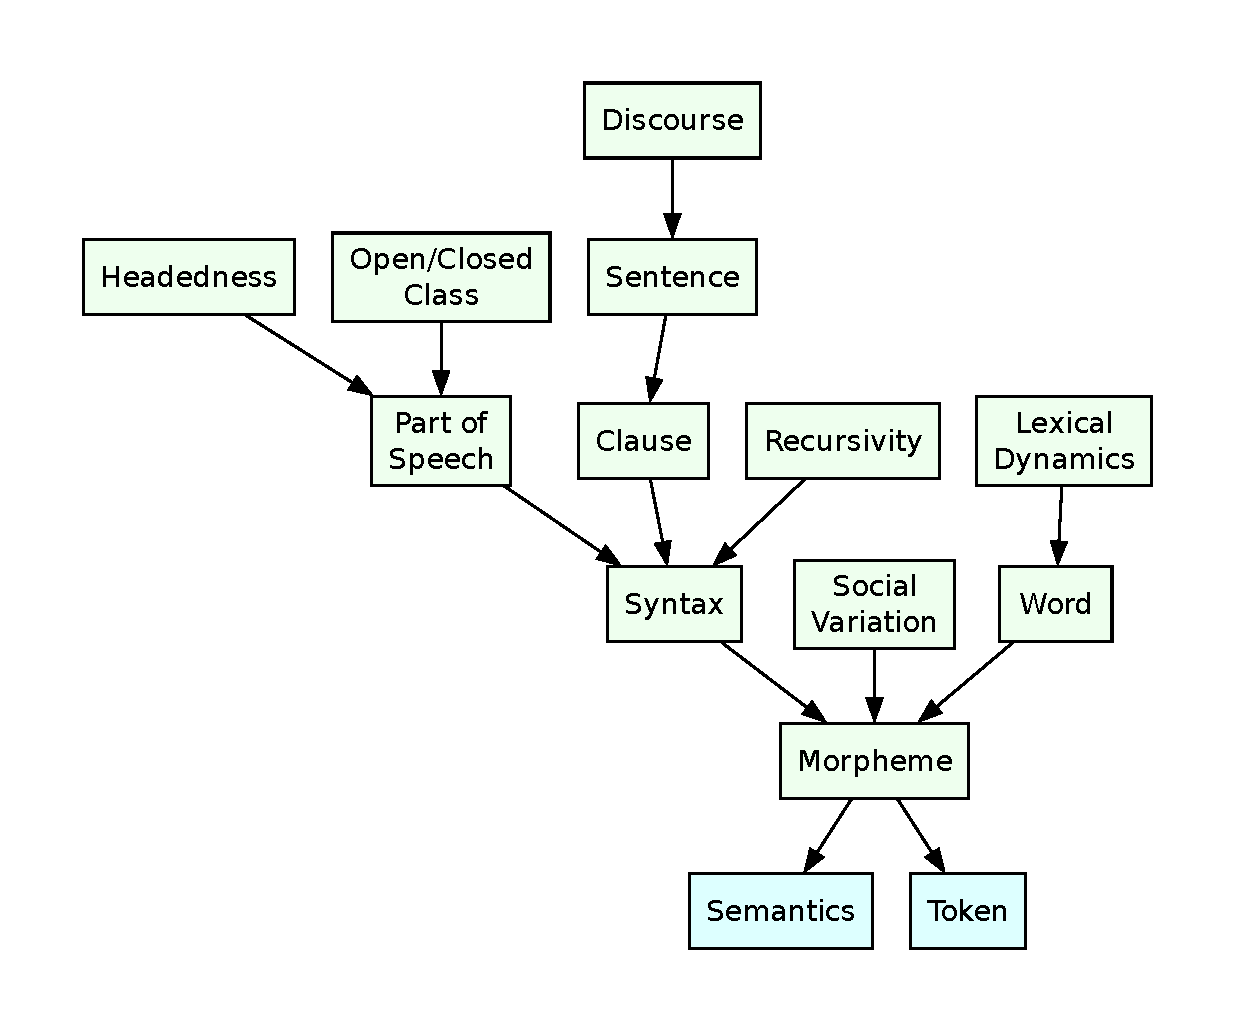
\includegraphics[width=0.85\linewidth]{assets/linguistic-dag}
  \caption{%
    Hierarchy of linguistic concepts.
    $X\rightarrow Y$ can be read as ``the definition of $X$ presupposes $Y$ being defined'' or roughly ``$X$ depends on $Y$''.
    The only concepts whose existence is established in emergent language are \emph{semantics} and \emph{token}.}
  \unskip\label{fig:linguistic-dag}
\end{figure}

Thus, I decided to pursue establishing a method to show the existence of and identify morphemes and syntax---the backbone of the hierarchy depicted in \Cref{fig:linguistic-dag}, which is likely the most that can be done toward developing a metric of linguistic similarity in the scope of this thesis.
Nevertheless, the proposed algorithms still fit well within this thesis' theme of pioneering accessible general purpose in methods in emergent communication that permit the direct comparison of emergent languages across a wide of environment and implementations.
